
\documentclass[a4paper,14pt]{extreport} % формат документа

%\documentclass[utf8x, 14pt]{G7-32}
\usepackage[warn]{mathtext}
\usepackage{amsmath}
\usepackage{cmap} % поиск в ПДФ
\usepackage[T2A]{fontenc} % кодировка
\usepackage[utf8]{inputenc} % кодировка исходного текста
\usepackage[english,russian]{babel} % локализация и переносы
\usepackage[left = 2cm, right = 1cm, top = 2cm, bottom = 2 cm]{geometry} % поля
\usepackage{listings}
\usepackage{graphicx} % для вставки рисунков
\usepackage{amsmath}
\usepackage{float}
\usepackage{longtable}
\usepackage{multirow}
\usepackage{pdfpages}
\graphicspath{{pictures/}}
\DeclareGraphicsExtensions{.pdf,.png,.jpg}
\newcommand{\anonsection}[1]{\section*{#1}\addcontentsline{toc}{section}{#1}}

\begin{document}
	
\begin{titlepage}
	
	\begin{table}[H]
		\centering
		\footnotesize
		\begin{tabular}{cc}
			\multirow{8}{*}{
\includegraphics[scale=0.35]{bmstu.jpg}}
			& \\
			& \\
			& \textbf{Министерство науки и высшего образования Российской Федерации} \\
			& \textbf{Федеральное государственное бюджетное образовательное учреждение} \\
			& \textbf{высшего образования} \\
			& \textbf{<<Московский государственный технический} \\
			& \textbf{университет имени Н.Э. Баумана>>} \\
			& \textbf{(МГТУ им. Н.Э. Баумана)} \\
		\end{tabular}
	\end{table}
	
	\vspace{-1.5cm}
	
	\begin{flushleft}
		\rule[-1cm]{\textwidth}{3pt}
		\rule{\textwidth}{1pt}
	\end{flushleft}
	
	\begin{flushleft}
		\small
		ФАКУЛЬТЕТ
		\underline{<<Информатика и системы управления>>\ \ \ \ \ \ \ 
			\ \ \ \ \ \ \ \ \ \ \ \ \ \ \ \ \ \ \ \ \ \ \ \ \ \ \ \ \ \ \ 
			\ \ \ \ \ \ \ \ \ \ \ \ \ \ \ } \\
		КАФЕДРА
		\underline{<<Программное обеспечение ЭВМ и
			информационные технологии>>
			\ \ \ \ \ \ \ \ \ \ \ \ \ \ \ \ \ \ \ \ }
	\end{flushleft}
	
	\vspace{2cm}
	
	\begin{center}
		\textbf{Лабораторная работа № 8} \\
		\textbf{Дисциплина:}  Компьютерные сети.  \\
		\textbf{Тема} 
		Изучение протоколов динамической \\ маршрутизации RIPv2 и OSPF в сетевом симуляторе\\
		\textbf{Вариант №15} \\
	\end{center}

    \vspace{4cm}
    
	\begin{flushright}
		\begin{tabular}{rr}
			\textbf{Студент} & Неклепаева А.Н. \\
			\textbf{Группа} & ИУ7-73Б \\
			\textbf{Преподаватель} & Рогозин Н.О.   \\
		\end{tabular}
	\end{flushright}
	
	\vspace{7cm}
	
	\begin{center}
		Москва, 2020 г.
	\end{center}
	
\end{titlepage}

\textbf{Задача:} 

I. Назначить адреса подсетей:

a) Подсеть 1: 192.168.x.0 /24

b) Подсеть 2: 192.168.x+1.0 /24

c) Подсеть 3: 192.168.x+2.0 /24

d) Подсеть 4: 192.168.x+3.0 /24

e) Подсеть 5 (В задаче III): 192.168.x+10.0 /24

II. Настроить динамическую маршрутизацию в прилагаемом .pkt файле на стенде I через протокол RIPv2 так, чтобы пинг любым хостом или маршрутизатором любого другого хоста или маршрутизатора был успешным.

Представить отдельным .pkt файлом. 

III. Настроить динамическую маршрутизацию в сети в прилагаемом .pkt файле на стенде II через протокол OSPF так, чтобы пинг любым хостом или маршрутизатором любого другого хоста или маршрутизатора был успешным. Разделить при этом сеть на области OSPF в соответствии со схемой. Выполнить указания в лабораторной работе.

Представить отдельным .pkt файлом. 

\textbf{Результаты работы:}

I. Разделение на подсети на стенде I.

На рис. \ref{fig:podseti1} указаны диапазоны адресов для каждой подсети.

\begin{figure}[H]
	\centering
	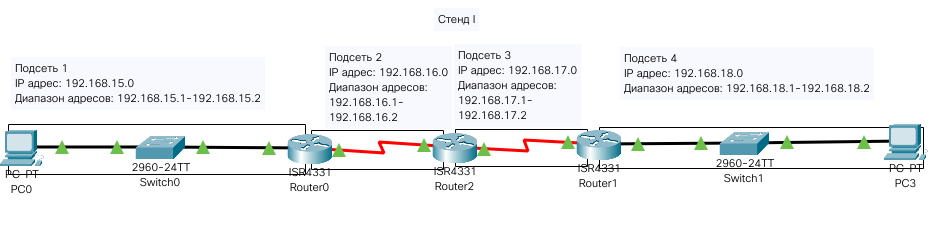
\includegraphics[width=1\linewidth]{podseti1}
	\caption{}
	\label{fig:podseti1}
\end{figure}


Разделение на подсети на стенде II.

На рис. \ref{fig:podseti2} указаны диапазоны адресов для каждой подсети.

\begin{figure}[H]
	\centering
	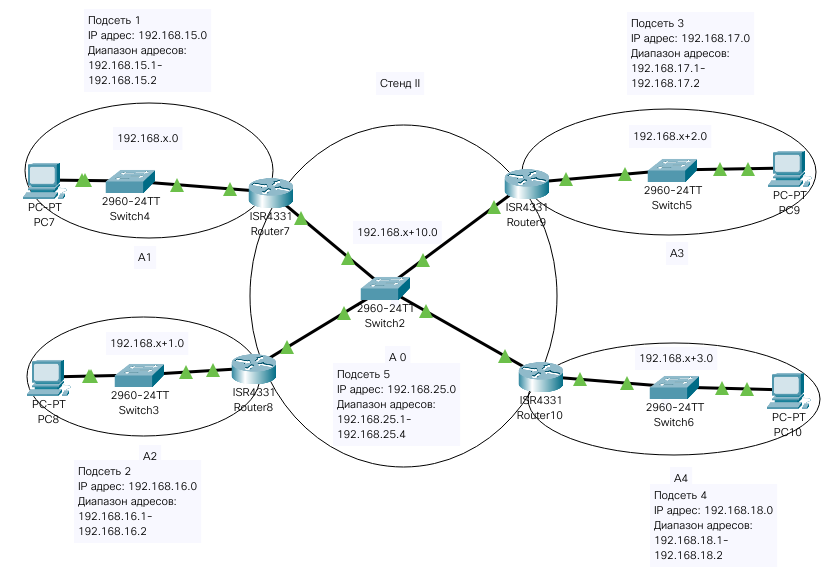
\includegraphics[width=1\linewidth]{podseti2}
	\caption{}
	\label{fig:podseti2}
\end{figure}

II. Настройка динамической маршрутизации на
стенде I через протокол RIPv2. 

Были добавлены сети, интерфейсы в которых будут использоваться настраиваемым маршрутизатором для рассылки маршрутной информации.

Для этого использовались команды, представленные ниже.

В режиме конфигурации:

router rip - команда перехода к режиму конфигурации маршрутизатора и настройки протокола RIP

В режиме конфигурации маршрутизатора:

network network\underline{ }num
, где network\underline{ }num - адрес сети
позволяет добавить сеть/диапазон адресов, который будет использоваться для рассылки обновлений RIP.

Для включения бесклассовой маршрутизации необходимо подключить модуль RIPv2.

В режиме конфигурации маршрутизатора и настройки RIP:
version 2 - изменение версии RIP на RIPv2

Пример настройки роутера Router0 показан на рис. \ref{fig:com}.

\begin{figure}[H]
	\centering
	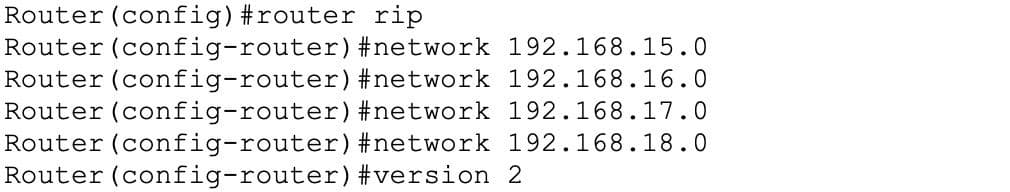
\includegraphics[width=1\linewidth]{com}
	\caption{}
	\label{fig:com}
\end{figure}

Настройка выполняется аналогично для остальных маршрутизаторов.

Пинг компьютером PC0 компьютера PC3 показан на рис. \ref{fig:ping1}.

\begin{figure}[H]
	\centering
	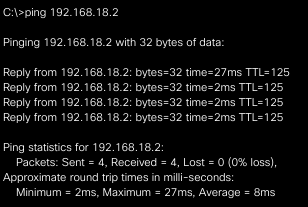
\includegraphics[width=0.7\linewidth]{ping1}
	\caption{}
	\label{fig:ping1}
\end{figure}

Пинг маршрутизатором Router0 маршрутизатора Router3 показан на рис. \ref{fig:ping2}.

\begin{figure}[H]
	\centering
	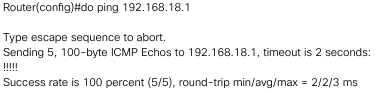
\includegraphics[width=1\linewidth]{ping2}
	\caption{}
	\label{fig:ping2}
\end{figure}

III. Настройка динамической маршрутизации на
стенде II через протокол OSPF.
\\

Команды для настройки роутеров.

router ospf 1 - команда позволяет перейти в режим конфигурирования маршрутизатора и настройки протокола ospf с идентификатором процесса равным 1. Идентификатор должен совпадать на всех устройствах.

В режиме конфигурирования маршрутизатора выполняется команда

network network-address wildcard-mask area\underline{ }num

где network-address- номер сети, 
wildcard-mask - маска, обратная маске подсети
area\underline{ }num - номер области ospf

Для обеспечения базовых средств безопасности необходимо настроить аутентификацию. 

Для включения аутентификации на основе пароля используются следующие команды:

ip ospf authentication-key key (для конкретного интерфейса)

area area-id authentication (для команды "router ospf <process-id>")

Настройка роутера Router7 показана на рис. \ref{fig:rout}.

\begin{figure}[H]
	\centering
	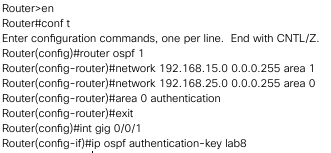
\includegraphics[width=0.7\linewidth]{rout}
	\caption{}
	\label{fig:rout}
\end{figure}

Для остальных роутеров настройка проводилась по аналогии.

Пинг компьютером PC7 компьютера PC10 показан на рис. \ref{fig:ping3}.

\begin{figure}[H]
	\centering
	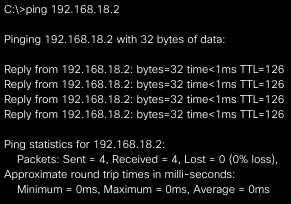
\includegraphics[width=0.7\linewidth]{ping3}
	\caption{}
	\label{fig:ping3}
\end{figure}

Пинг маршрутизатором Router8 маршрутизатора Router9 показан на рис. \ref{fig:ping4}.

\begin{figure}[H]
	\centering
	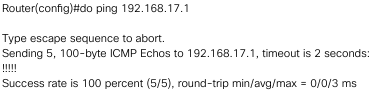
\includegraphics[width=1\linewidth]{ping4}
	\caption{}
	\label{fig:ping4}
\end{figure}

Для отображения информации о статусе соседних устройств можно использовать команду

sh ip ospf neighbor 

Вывод команды sh ip ospf neighbor для роутера Router8 показан на рис. \ref{fig:st}.

\begin{figure}[H]
	\centering
	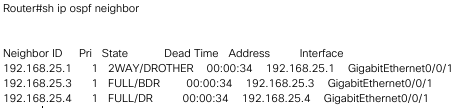
\includegraphics[width=1\linewidth]{st}
	\caption{}
	\label{fig:st}
\end{figure}

Роутер Router10 выбран как  DR. Роутер Router9 выбран как  BDR (резервный назначенный маршрутизатор). 

Так как все маршрутизаторы соединены с различными зонами, они все имеют статус ABR  (граничный маршрутизатор области).

\end{document}
	